\documentclass{beamer}
\usepackage[utf8]{inputenc}
\usepackage[english]{babel}
\usepackage[T1]{fontenc}
\usepackage[inline]{asymptote}
\usepackage{pgfplots}
\pgfplotsset{compat=1.5} 
\usepgfplotslibrary{statistics}
\usepackage{graphicx}
\usepackage{slide_helper}

\title[MA205 - Section 2.2]{Histograms}

\newcommand{\textsep}{\vspace{0.5mm}}

\begin{document}
\begin{frame}
\titlepage
\end{frame}

\begin{frame}
\begin{definition}
A \textbf{histogram} is a graph consisting of bars of equal width drawn adjacent to each other. The horizontal scale represents classes of quantitative data values, and the vertical scale represents frequencies. The heights of the bars correspond to the frequency values.
\end{definition}

\onslide<2->
\begin{block}{Important Uses}
\begin{itemize}
\item<2-> Visually displays the shape of the distribution of the data.
\item<3-> Shows the location of the center of the data.
\item<4-> Shows the spread of the data.
\item<5-> Identifies outliers.
\end{itemize}
\end{block}
\end{frame}

\begin{frame}
\begin{example}
The table contains drive-through service times, in seconds, for McDonald's.
\begin{center}
\begin{tabular}{rrrrrrrrrrrr}
107 & 139 & 197 & 209 & 281 & 254 & 163 & 150 & 127 & 308 & 206 & 187 \\
169 &  83 & 127 & 133 & 140 & 143 & 130 & 144 &  91 & 113 & 153 & 255 \\
252 & 200 & 117 & 167 & 148 & 184 & 123 & 153 & 155 & 154 & 100 & 117 \\
101 & 138 & 186 & 196 & 146 &  90 & 144 & 119 & 135 & 151 & 197 & 171 \\
\end{tabular}
\end{center}
The histogram for this data is:

\vspace{-4mm}
\begin{center}
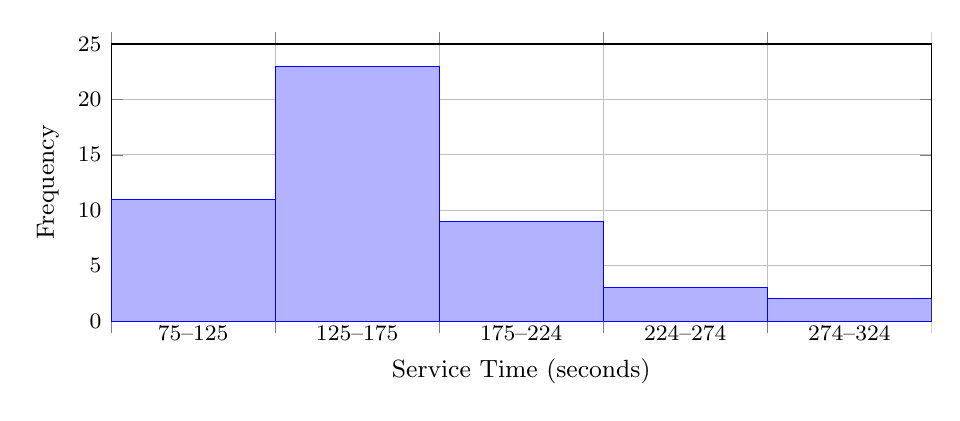
\begin{tikzpicture}
\begin{axis}[
small,
height=5.1cm,
width=12.0cm,
enlarge x limits=false,
enlarge y limits=false,
ybar interval,
ymajorgrids=true,
ylabel={Frequency},
xlabel={Service Time (seconds)},
x tick label style={rotate=0,anchor=center},
%xtick={120,140,...,1000},
ytick={0,5,...,1000},
ymin=0,
ymax=25,
%xmin=120,
%xmax=280,
xticklabel style={/pgf/number format/.cd,fixed,precision=0},
xticklabel=
\pgfmathprintnumber\tick--\pgfmathprintnumber\nexttick
]
\addplot+ [hist={bins=5, data min=75, data max=324}]
table [row sep=\\,y index=0] {
data\\
107 \\ 139 \\ 197 \\ 209 \\ 281 \\ 254 \\ 163 \\ 150 \\ 127 \\ 308 \\ 206 \\ 187 \\
169 \\  83 \\ 127 \\ 133 \\ 140 \\ 143 \\ 130 \\ 144 \\  91 \\ 113 \\ 153 \\ 255 \\
252 \\ 200 \\ 117 \\ 167 \\ 148 \\ 184 \\ 123 \\ 153 \\ 155 \\ 154 \\ 100 \\ 117 \\
101 \\ 138 \\ 186 \\ 196 \\ 146 \\  90 \\ 144 \\ 119 \\ 135 \\ 151 \\ 197 \\ 171 \\
};
\end{axis}
\end{tikzpicture}
\end{center}
\end{example}
\end{frame}

\begin{frame}
\begin{definition}
A \textbf{relative frequency histogram} has the same shape and scale as a histogram, but the vertical scales uses relative frequency instead of actual frequencies.
\end{definition}\pause

\begin{example}
The relative frequency histogram for the McDonald's data is:
\begin{center}
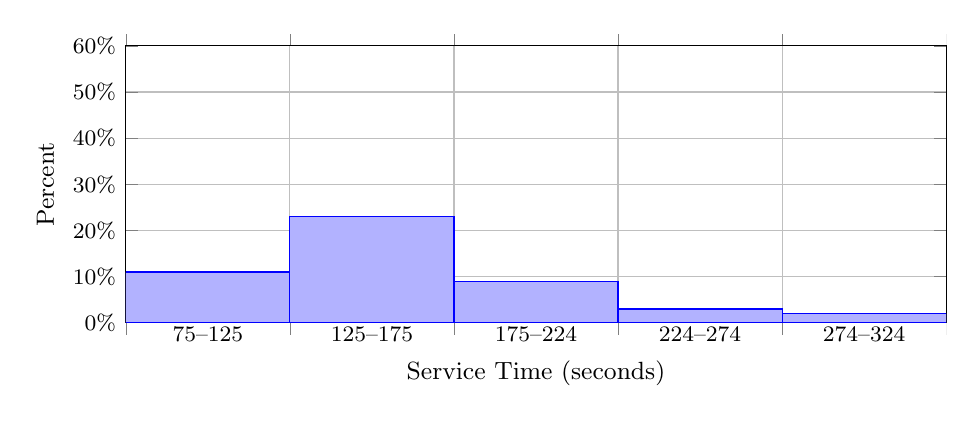
\begin{tikzpicture}
\begin{axis}[
small,
height=5.1cm,
width=12.0cm,
enlarge x limits=false,
enlarge y limits=false,
ybar interval,
ymajorgrids=true,
ylabel={Percent},
xlabel={Service Time (seconds)},
x tick label style={rotate=0,anchor=center},
%xtick={120,140,...,1000},
ytick={0,10,...,1000},
ymin=0,
ymax=60,
%xmin=120,
%xmax=280,
xticklabel style={/pgf/number format/.cd,fixed,precision=0},
xticklabel=
\pgfmathprintnumber\tick--\pgfmathprintnumber\nexttick,
yticklabel style={/pgf/number format/.cd,fixed,precision=0},
yticklabel=
\pgfmathprintnumber\tick\%
]
\addplot+ [hist={bins=5, data min=75, data max=324}]
table [row sep=\\,y index=0] {
data\\
107 \\ 139 \\ 197 \\ 209 \\ 281 \\ 254 \\ 163 \\ 150 \\ 127 \\ 308 \\ 206 \\ 187 \\
169 \\  83 \\ 127 \\ 133 \\ 140 \\ 143 \\ 130 \\ 144 \\  91 \\ 113 \\ 153 \\ 255 \\
252 \\ 200 \\ 117 \\ 167 \\ 148 \\ 184 \\ 123 \\ 153 \\ 155 \\ 154 \\ 100 \\ 117 \\
101 \\ 138 \\ 186 \\ 196 \\ 146 \\  90 \\ 144 \\ 119 \\ 135 \\ 151 \\ 197 \\ 171 \\
};
\end{axis}
\end{tikzpicture}
\end{center}
\end{example}
\end{frame}

\begin{frame}[fragile]
\begin{block}{Normal Distribution}
% Gauss function, parameters mu and sigma
\newcommand\gauss[2]{24500/(#2*sqrt(2*pi))*exp(-((x-#1)^2)/(2*#2^2))} % chktex 36

\begin{tikzpicture}
\pgfplotsset{set layers}
\begin{axis}[
small,
height=6.4cm,
width=12.0cm,
enlarge x limits=false,
enlarge y limits=false,
ybar interval,
ymajorgrids=true,
ylabel={Percent},
xlabel={Service Time (seconds)},
%x tick label style={rotate=0,anchor=center},
xtick={10,20,...,500},
%ytick={0,10,...,1000},
xmin=0,
xmax=190,
ymin=0,
ymax=550
%xticklabel style={/pgf/number format/.cd,fixed,precision=0},
%xticklabel=
%\pgfmathprintnumber\tick--\pgfmathprintnumber\nexttick,
%yticklabel style={/pgf/number format/.cd,fixed,precision=0},
%yticklabel=
%\pgfmathprintnumber\tick\%
]
\addplot+ [hist={bins=75}]
table [y=nums] {randn.dat};
\end{axis}

\begin{axis}[
small,
height=6.4cm,
width=12.0cm,
enlarge x limits=false,
enlarge y limits=false,
xticklabels={},yticklabels={},
xmin=0,
xmax=190,
ymin=0,
ymax=550]
\addplot[domain={10:180},samples=100, red, dashed, thick]{\gauss{99.79922645}{25.01315794}};
\end{axis}
\end{tikzpicture}
\end{block}\pause

\begin{block}{Note}
Many statistical methods require that sample data come from a population having a distribution that is approximately a normal distribution.
\end{block}
\end{frame}

\begin{frame}
\begin{block}{Uniform Distribution}
\begin{tikzpicture}
\begin{axis}[
small,
height=8.1cm,
width=12.0cm,
enlarge x limits=false,
enlarge y limits=false,
ybar interval,
ymajorgrids=true,
ylabel={Frequency},
xlabel={},
x tick label style={rotate=0,anchor=center},
%xtick={0,1,2,3,4,5,6,7,8,9},
%ytick={0,1,...,10},
ymin=0,
ymax=1100,
%xmin=0,
%xmax=9,
%xticklabel style={/pgf/number format/.cd,fixed,precision=0},
%xticklabel=
%\pgfmathprintnumber\tick--\pgfmathprintnumber\nexttick,
%yticklabel style={/pgf/number format/.cd,fixed,precision=0},
%yticklabel=
%\pgfmathprintnumber\tick\%
]
\addplot+ [hist={bins=10, data min=0, data max=10}]
table [y=nums] {randu.dat};
\end{axis}
\end{tikzpicture}
\end{block}
\end{frame}

\begin{frame}
\begin{block}{Skew Right}
\begin{tikzpicture}
\begin{axis}[
small,
height=8.1cm,
width=12.0cm,
enlarge x limits=false,
enlarge y limits=false,
ybar interval,
ymajorgrids=true,
ylabel={Frequency},
xlabel={},
x tick label style={rotate=0,anchor=center},
xtick={0,10,...,60},
%ytick={0,1,...,10},
ymin=0,
ymax=700,
%xmin=0,
%xmax=9,
%xticklabel style={/pgf/number format/.cd,fixed,precision=0},
%xticklabel=
%\pgfmathprintnumber\tick--\pgfmathprintnumber\nexttick,
%yticklabel style={/pgf/number format/.cd,fixed,precision=0},
%yticklabel=
%\pgfmathprintnumber\tick\%
]
\addplot+ [hist={bins=60, data min=0, data max=60}]
table [y=nums] {randsr.dat};
\end{axis}
\end{tikzpicture}
\end{block}
\end{frame}

\begin{frame}
\begin{block}{Skew Right}
\begin{tikzpicture}
\begin{axis}[
small,
height=8.1cm,
width=12.0cm,
enlarge x limits=false,
enlarge y limits=false,
ybar interval,
ymajorgrids=true,
ylabel={Frequency},
xlabel={},
x tick label style={rotate=0,anchor=center},
xtick={0,10,...,60},
%ytick={0,1,...,10},
ymin=0,
ymax=700,
%xmin=0,
%xmax=9,
%xticklabel style={/pgf/number format/.cd,fixed,precision=0},
%xticklabel=
%\pgfmathprintnumber\tick--\pgfmathprintnumber\nexttick,
%yticklabel style={/pgf/number format/.cd,fixed,precision=0},
%yticklabel=
%\pgfmathprintnumber\tick\%
]
\addplot+ [hist={bins=60, data min=0, data max=60}]
table [y=nums] {randsl.dat};
\end{axis}
\end{tikzpicture}
\end{block}
\end{frame}

\begin{frame}
\begin{block}{Note}
\begin{columns}
\begin{column}{0.18\textwidth}
Skewed to the left resembles the toes on your left foot.
\end{column}
\begin{column}{0.55\textwidth}
\includegraphics[width=\textwidth]{feet.png}
\end{column}
\begin{column}{0.18\textwidth}
Skewed to the right resembles the toes on your right foot.
\end{column}
\end{columns}
\end{block}\pause

\begin{definition}
If the distribution of data is skewed to the left or skewed to the right, it is called \textbf{skewed}.
\end{definition}
\end{frame}
\end{document}
